\chapter{Detalles de Implementación y Experimentos}\label{chapter:implementation}
 
\section{Herramientas y tecnologías utilizadas}
 
\subsection{The Unity Engine}
 
Unity es una plataforma de desarrollo 3D en tiempo real que consta de un motor de renderizado y de física, así como de una interfaz gráfica de usuario llamada Unity Editor. Unity ha recibido una amplia adopción en los sectores del juego, la arquitectura, la ingeniería y la construcción, el automóvil y el cine, y es utilizado por una gran comunidad de desarrolladores de juegos para realizar una gran variedad de simulaciones interactivas, que van desde pequeños juegos para móviles y navegadores hasta juegos de consola de alto presupuesto y experiencias de de realidad virtual.
 
\subsection{Tensorflow}
 
TensorFlow es una interfaz para expresar algoritmos de aprendizaje automático y una implementación para ejecutar dichos algoritmos. Un cómputo expresado con TensorFlow se puede ejecutar con poco o ningún cambio en una amplia variedad de sistemas heterogéneos, desde dispositivos móviles como teléfonos y tabletas hasta sistemas distribuidos a gran escala de cientos de máquinas y miles de dispositivos computacionales como tarjetas GP. El sistema es flexible y se puede usar para expresar una amplia variedad de algoritmos, incluidos algoritmos de entrenamiento e inferencia para modelos de redes neuronales profundas, y se ha usado para realizar investigaciones y para implementar sistemas de aprendizaje automático en producción en más de una docena de áreas de ciencias de la computación y otros campos, incluidos el reconocimiento de voz, la visión por computadora, la robótica, la recuperación de información, el procesamiento del lenguaje natural, la extracción de información geográfica y el descubrimiento computacional de fármacos. (\cite{tensorflow2015-whitepaper}).
 
\subsection{PyTorch}
 
PyTorch es un framework de aprendizaje automático de código abierto basado en el lenguaje de programación Python y la biblioteca Torch. Es una de las plataformas preferidas para la investigación del aprendizaje profundo. El marco está construido para acelerar el proceso entre la creación de prototipos de investigación y el despliegue. (\cite{NEURIPS2019_9015})
 
\subsection{Unity ML-Agents Toolkit}
 
El Unity Machine Learning Agents Toolkit (ML-Agents) es un proyecto de código abierto que permite que los juegos y las simulaciones sirvan como entornos para el entrenamiento de agentes inteligentes. Proporciona implementaciones (basadas en TensorFlow y PyTorch) de algoritmos de última generación para permitir a los desarrolladores de juegos y aficionados entrenar fácilmente agentes inteligentes para juegos 2D, 3D y VR/AR. Los investigadores también pueden utilizar la API de Python, que es muy fácil de usar, para entrenar a los agentes mediante el aprendizaje por refuerzo, el aprendizaje por imitación, la neuroevolución o cualquier otro método. Estos agentes entrenados pueden ser utilizados para múltiples propósitos, incluyendo el control del comportamiento de los NPCs (en una variedad de escenarios tales como multi-agentes y adversarios), pruebas automatizadas de construcciones de juegos y evaluación de diferentes decisiones de diseño de juegos antes de su lanzamiento. El ML-Agents Toolkit es mutuamente beneficioso tanto para los desarrolladores de juegos como para los investigadores de IA, ya que proporciona una plataforma central en la que los avances en IA pueden ser evaluados en los ricos entornos de Unity y luego se hacen accesibles a las comunidades más amplias de investigadores y desarrolladores de juegos. 
 
Las características del kit de herramientas incluyen un conjunto de entornos de ejemplo, algoritmos RL de última generación como Soft Actor-Critic (SAC) (\cite{haarnoja2018soft}) y Proximal Policy Optimization (PPO) (\cite{schulman2017proximal})  entre otros.
 
\section{Implementación de UTHOPIA}
 
Unity ML expone un API para comunicar Unity a la biblioteca de Python donde realmente están los algoritmos. Unity funciona como un simulador que brinda las observaciones visuales, físicas entre otras. Esto permite concentrarse en desarrollar la parte referida a los juegos, cómo se perciben y cómo se controlan por un lado, y probar algoritmos o hacer un uso personalizado de la biblioteca de ml-agents de forma separada.
 
\subsection{Interfaz entre UTHOPIA y Unity ML}
 
Para comenzar la implementación lo primero se hizo fue heredar de la clase \lstinline{UnityML.Agente} y sobrescribir sus métodos. En Uthopia se ha utilizado esta clase para construir el \lstinline{AgentManager}, un controlador que normaliza tanto observaciones como acciones para que sea fácil de trabajar a la hora de crear los juegos y menos propenso a errores. De esta forma se puede transformar la entrada en una clase conocida \lstinline{Uthopia.InputData} y se limita el acceso al sistema de recompensas restringiendo a su uso a los estados terminales de los juegos: las victorias o las derrotas. 
 
\begin{lstlisting}[caption={Implementación de la clase \lstinline{AgentManager} la cual conecta a los agentes de Unity ML Toolkit con los juegos de UTHOPIA}]
    public class AgentManager: Agent
    {
        public override void Initialize()
        {
            uthopia.Game.instance.Initialize(seed);
 
            // Win Event
            uthopia.Game.instance.onWin.AddListener(
                () => { 
                    AddReward(1); 
                    EndEpisode();
                });
 
            // GameOver event
            uthopia.Game.instance.onLose.AddListener(
                () => { 
                    AddReward(-1); 
                    EndEpisode(); 
                });
        }
 
        public override void OnEpisodeBegin()
        {
            uthopia.Game.instance.OnEpisodeBegin();
        }
 
        public override void OnActionReceived(ActionBuffers actions)
        {
            uthopia.Game.instance.OnInputReceived(new uthopia.InputData(actions.DiscreteActions.Array));
        }
    }
\end{lstlisting}

\subsection{Implementación de Juegos}
 
La clase \lstinline{Game} creada permite crear juegos a partir de la implementación de sus métodos. El ciclo de vida de un juego comienza en \lstinline{Initialize}, luego en cada inicio de episodio se invoca a \lstinline{OnEpisodeBegin}, y durante el episodio, cada vez que se reciben las acciones, se llama a \lstinline{OnInputReceived}. El juego termina si se llama \lstinline{Win} o \lstinline{Lose}, en cuyo caso UTHOPIA regresará a llamar \lstinline{OnEpisodeBegin} dando inicio a otra instancia del juego, o terminará con la fase que procede.
 
\begin{figure}[ht!]
    \centering
    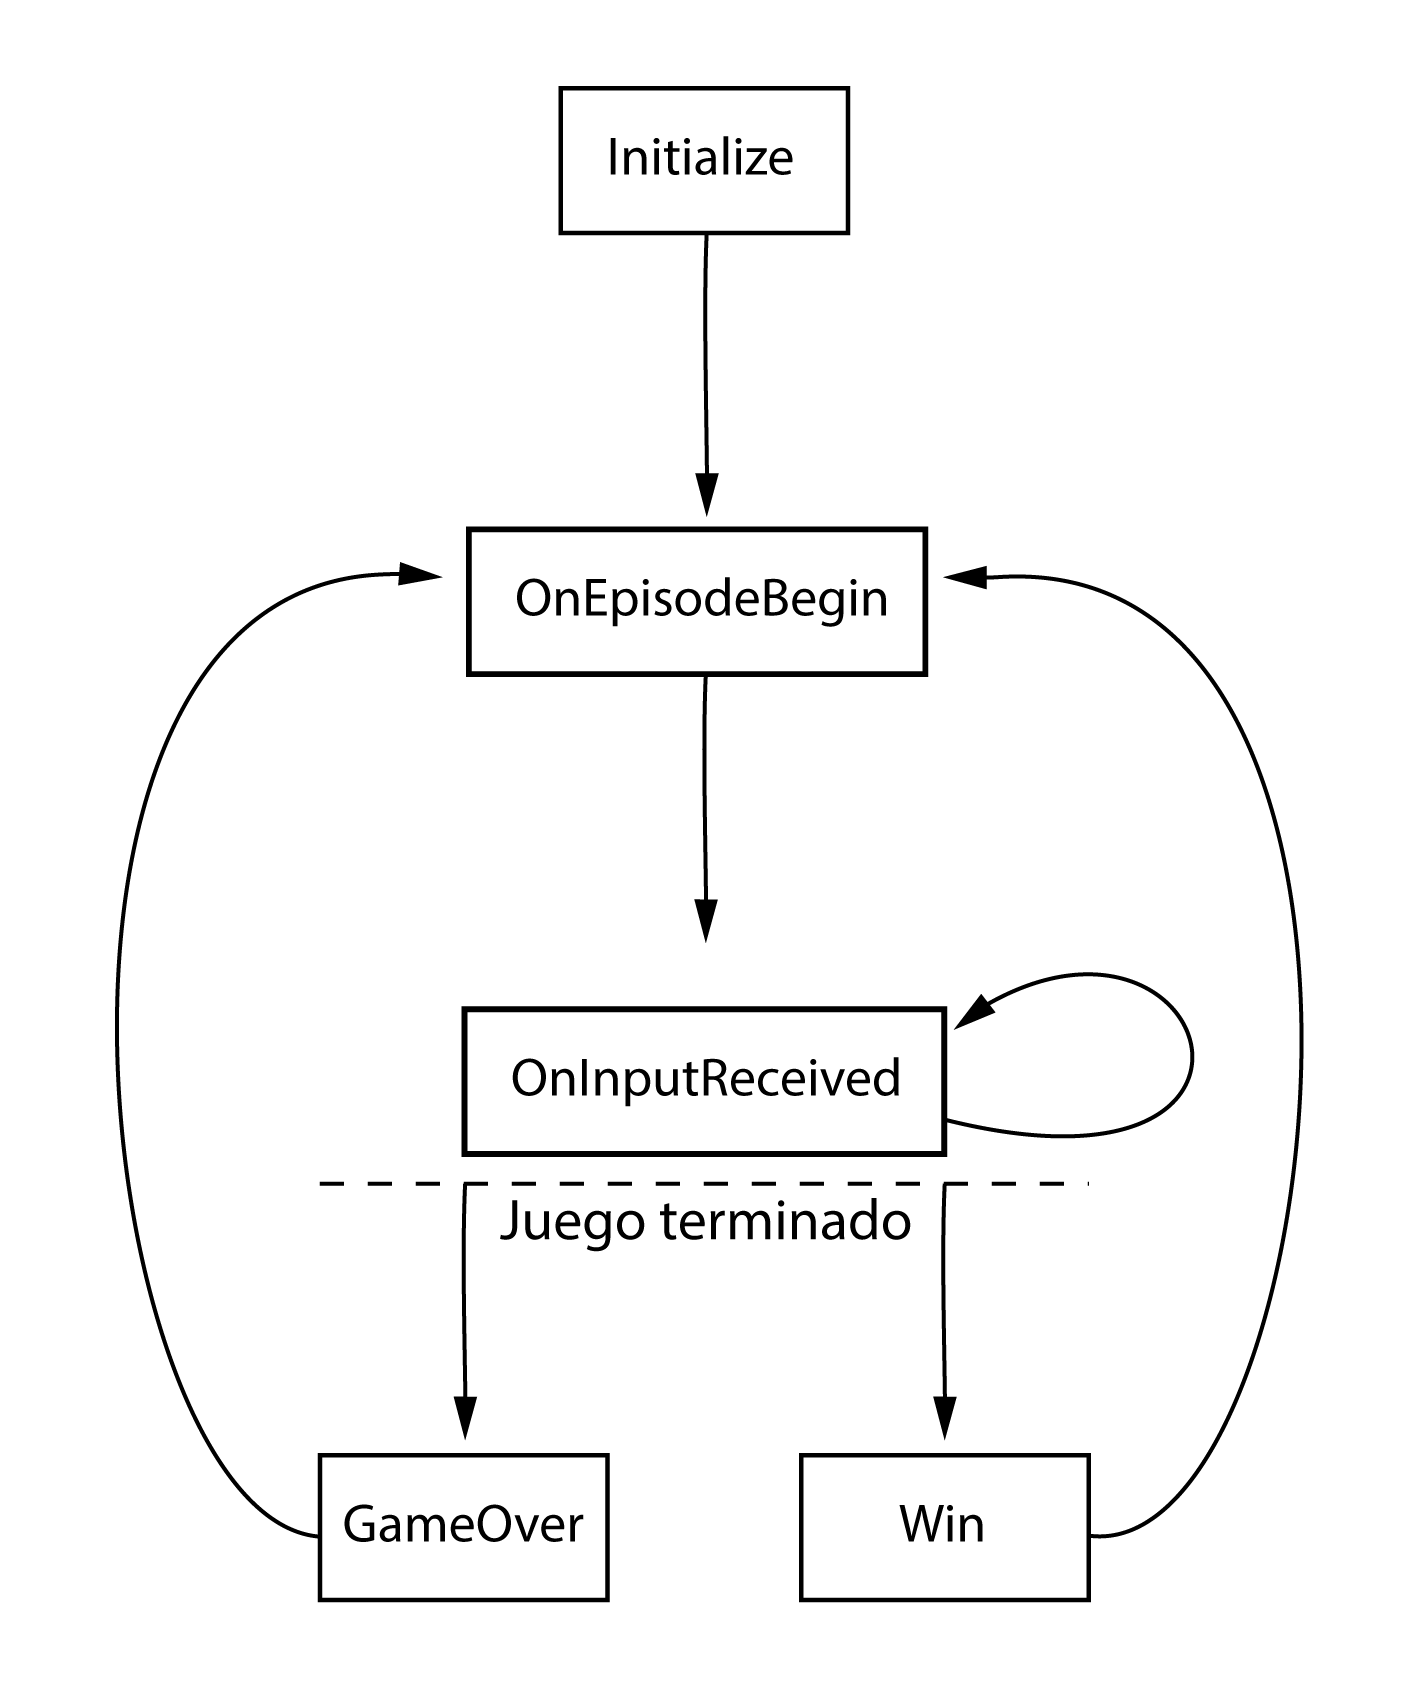
\includegraphics[width=0.7\textwidth]{Graphics/uthopia_game_flow.png}
    \caption{Diagrama del ciclo de un juego.}
    \label{fig:cicle-of-games}
\end{figure}
 
\vspace*{1cm}
 
\begin{lstlisting}[caption={Implementación de la clase \lstinline{Game} base para todos los juegos de UTHOPIA}]
    public abstract class Game : MonoBehaviour
    {
        private static Game _instance;
        public static Game instance {
            get {
                if (!_instance)
                {
                    _instance =  FindObjectOfType<Game>(true);
                }
                return _instance;
            }
        }
 
        public GameSettings settings { private set; get; }
        public int seed { private set; get; }
 
        public UnityEvent onWin;
        public UnityEvent onLose;
 
        public virtual void Initialize(int seed, GameSettings settings = null)
        {
            onWin.RemoveAllListeners();
            onLose.RemoveAllListeners();
            this.settings = settings;
            this.seed = seed;
        }
 
        public abstract void OnEpisodeBegin();
        public abstract void OnInputReceived(InputData input);
 
        protected void Win()
        {
            Camera.main.backgroundColor = Color.green;
            Invoke(nameof(RestartCamera), 0.1f);
            onWin.Invoke();
        }
 
        protected void Lose()
        {
            Camera.main.backgroundColor = Color.red;
            Invoke(nameof(RestartCamera), 0.1f);
            onLose.Invoke();
        }
 
        void RestartCamera() {
            Camera.main.backgroundColor = Color.black;
        }
    }
\end{lstlisting}
 
\subsection{La heurística para agentes humanos}
 
Para obtener las entradas del los agentes humanos mediante el teclado implementamos el método Heuristic el cual permite agregar acciones de forma determinista. Esto facilita que cuando el Agente está en modo \textit{Heuristic Only} las personas puedan participar en la prueba directamente.
 
\vspace*{1cm}
 
\begin{lstlisting}[caption={Implementación de la asignación de acciones heurística para captar la entrada de los agentes humanos.}]
    public override void Heuristic(in ActionBuffers actionsOut)
    {
        // DIRECTIONAL
        var discrete = actionsOut.DiscreteActions;
 
        if (Input.GetKey(KeyCode.A) != Input.GetKey(KeyCode.D))
        {
            discrete[0] = Input.GetKey(KeyCode.A) ? 1 : 2;
        }
        else discrete[0] = 0;
 
        if (Input.GetKey(KeyCode.W) != Input.GetKey(KeyCode.S))
        {
            discrete[1] = Input.GetKey(KeyCode.S) ? 1 : 2;
        }
        else discrete[1] = 0;
 
        // EX ACTIONS
        discrete[2] = (Input.GetKey(KeyCode.U) ? 1 : 0);
        discrete[3] = (Input.GetKey(KeyCode.I) ? 1 : 0);
        discrete[4] = (Input.GetKey(KeyCode.O) ? 1 : 0);
        discrete[5] = (Input.GetKey(KeyCode.P) ? 1 : 0);
    }
\end{lstlisting} 
 
\subsection{Configuración de los componentes de UTHOPIA y Unity ML}
 
Desde el editor, en el componente de \lstinline{BehaviorParameters}, se deben configurar los espacios de acción  (\ref{fig:unity-editor-1}) y los sensores para la observación.

De las $6$ acciones admitidas, las primeras dos son de semánticamente las de dirección y aceptan $3$ valores discretos ${{0,1,2}}$ y el resto solo $2$ valores discretos ${{0,1}}$.
 
Además se agrega el componente de \lstinline{CameraSensor} para captar las observaciones visuales. Este sensor capta los píxeles de la cámara y los agrega al la lista de observaciones eviadas al receptor en python. 
 
\begin{figure}[ht!]
    \centering
    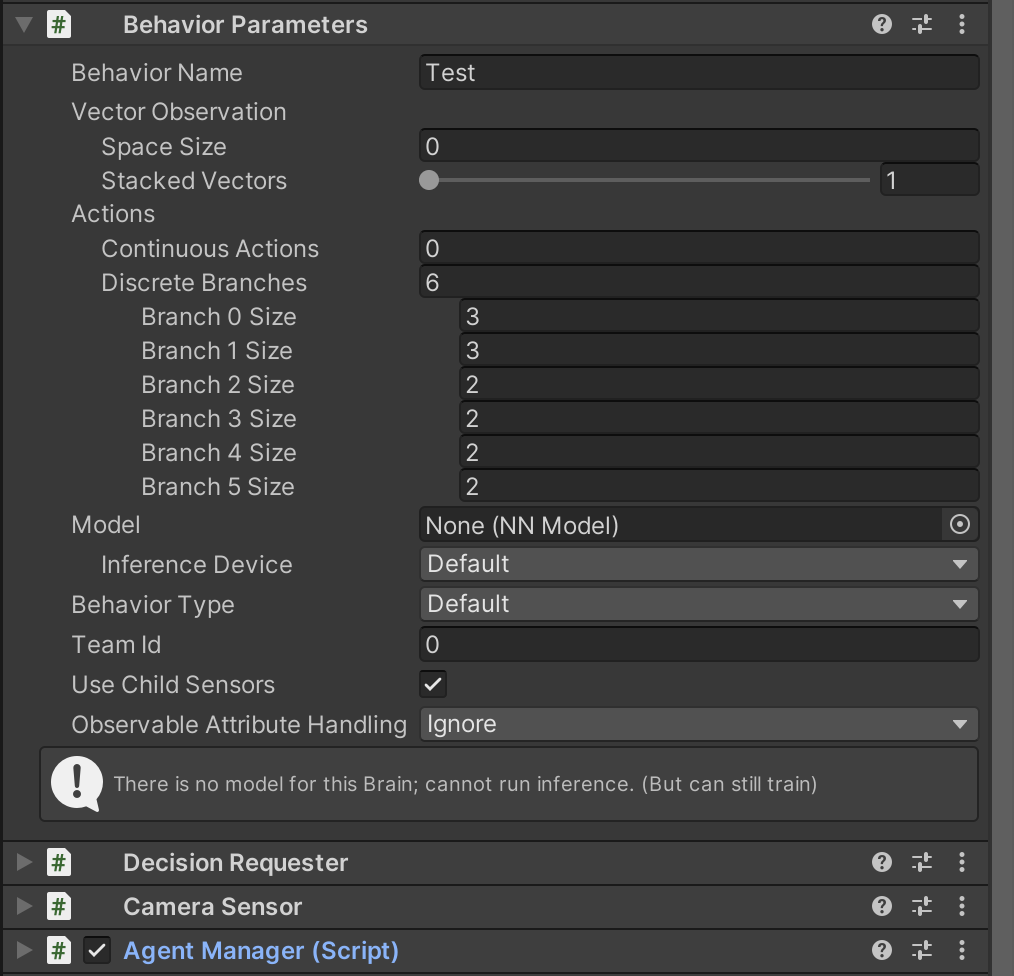
\includegraphics[width=0.7\textwidth]{Graphics/unity_editor.png}
    \caption{Configuración de componentes del \lstinline{GameObject AgentManager}.}
    \label{fig:unity-editor-1}
\end{figure}
 
\section{Ejemplo: Creación de un juego}
 
\lstinline{FindGoalGame} es un juego sencillo que trata sobre mover el objeto blanco y hacer que toque el objeto verde. Es uno de los juegos más básicos. La mera idea de mostrar dos objetos en pantalla debería inducir a los agentes a provocar su interacción en pocos intentos. 
 
\vspace*{1cm}
 
\begin{lstlisting}[caption={Ejemplo de implementación de un juego que trata sobre un objeto de color blanco que debe tocar al objeto verde.}]
    public class FindGoalGame : Game
    {
        public EntityController prefab;
        public float speedScale = 1;
 
        EntityController m_player;
        List<GameObject> m_createdObjects = new List<GameObject>();
 
        private void Update()
        {
            // Kepp player on camera
            if (m_player)
            {
                m_player.transform.position = m_player.position.InsideSquareBounds(15);
            }
        }
 
        public override void OnEpisodeBegin()
        {
            StopAllCoroutines();
 
            m_createdObjects.ForEach(g => ObjectPool.Set("entity", g.gameObject));
            m_createdObjects.Clear();
 
            // Spawn player
            var playerPos = Random.insideUnitCircle * 5;
            m_player = ObjectPool.Get("entity", prefab, Random.insideUnitCircle * 5, Quaternion.identity);
            m_player.Reset();
            m_player.SetColor(Color.white);
            m_player.speed = speedScale * 8;
 
            // Spawn goal
            for (var i = 0; i < 1; i++)
            {
                var randomPos = Random.insideUnitCircle * 10 * speedScale;
                var goal = ObjectPool.Get("entity", prefab, playerPos + randomPos, Quaternion.identity);
                goal.Reset();
                goal.SetColor(Color.green);
                goal.onCollisionEnter.RemoveAllListeners();
                goal.onCollisionEnter.AddListener(
                    collision =>
                    {
                        if (collision.gameObject == m_player.gameObject)
                        {
                            Win();
                        }
                    }
                    );
 
                goal.transform.position = goal.position.InsideSquareBounds(15);
                m_createdObjects.Add(goal.gameObject);
            }
            m_createdObjects.Add(m_player.gameObject);
        }
 
        public override void OnInputReceived(InputData input)
        {
            m_player.Move(input.direction);
        }
 
        
        public override InputActionMask GetInputMask()
        {
            return new InputActionMask(action5: false, action6: false, action7: false, action8: false);
        }
    }
\end{lstlisting}
 
Otros juegos similares pueden incluir obstáculos estáticos o móviles, otros objetivos, o presentar patrones particulares que requieren combinar diferentes razonamientos atómicos. Creando así variantes del mismo juego pero con ideas novedosas que requieran una nueva solución.

\section{Experimentos}
 
En los siguientes experimentos se hará una prueba a pequeña escala del proceso de evaluación de UTHOPIA. Se han creado $4$ juegos para la demostración y se comparará el desempeño entre $3$ personas y dos algoritmos de RL: Proximal Policy Optimization (PPO) y Soft Actor-Critic (SAC)..
 
El juego $1$ trata sobre alcanzar el objetivo verde con el objeto blanco. El juego $2$ (Figura \ref{fig:uthopia} a la derecha) consiste en alcanzar el objetivo verde evadiendo los obstáculos. El juego $1$ es una variante sin obstáculos del $2$. El juego $3$ (\ref{fig:uthopia_street}) consiste en tocar dos objetivos cruzando los obstáculos móviles. El juego $4$ (Figura \ref{fig:uthopia} a la izquierda) representa un problema de conteo, donde al tocar un objeto de un color, todos los objetos se mueven destruyéndose uno a uno contra el otro grupo.

Las $3$ personas fueron selecionadas al azar de entre los familares del autor y no conocían los juegos con antelación. La persona $1$ es un varón de $22$ años, la persona $2$ es una mujer de $64$ años y la persona $3$ es una chica de $20$ años. 

Los hiperparámetros utilizados para ambos algoritmos fueron seleccionados por defecto como son ofrecidos por Unity ML. Si bien un ajuste manual pudiese ayudarle a converger mejor, no es el objetivo del documento encontrar dichas combinaciones.
 
\vspace*{1cm}
 
\begin{lstlisting}[caption={Configuración de hiperparámetros para el agente con el algoritmo PPO}]
    behaviors:
        SimplePPO:
            trainer_type: ppo
            hyperparameters:
                batch_size: 10
                buffer_size: 100
                learning_rate: 3.0e-4
                beta: 5.0e-4
                epsilon: 0.2
                lambd: 0.99
                num_epoch: 3
                learning_rate_schedule: linear
                beta_schedule: constant
                epsilon_schedule: linear
            network_settings:
                normalize: false
                hidden_units: 128
                num_layers: 2
            reward_signals:
                extrinsic:
                    gamma: 0.99
                    strength: 1.0
            max_steps: 500000
            time_horizon: 64
            summary_freq: 10000
 
\end{lstlisting}
 
\vspace*{1cm}
 
\begin{lstlisting}[caption={Configuración de hiperparámetros para el agente con el algoritmo SAC}]
    behaviors:
        SimpleSAC:
            trainer_type: sac
            hyperparameters:
                learning_rate: 0.0003
                learning_rate_schedule: constant
                batch_size: 32
                buffer_size: 512
                buffer_init_steps: 10000
                tau: 0.005
                steps_per_update: 4.0
                save_replay_buffer: False
                init_entcoef: 0.5
            network_settings:
                normalize: false
                hidden_units: 128
                num_layers: 2
            reward_signals:
                extrinsic:
                    gamma: 0.99
                    strength: 1.0
            max_steps: 500000
            time_horizon: 64
            summary_freq: 10000
 
\end{lstlisting}
 
\subsection{Pasos para realizar la evaluación}
 
Como se indicó en (\ref{chapter:proposal:evaluation-flow}), la evaluación se realiza en dos fases: Preparación y Prueba. La transición entre ellas no es automática en la implementación que se ha realizado. 
 
Durante el experimento se realizaron las etapas de preparación contando 5 minutos. Para los humanos esto era en tiempo real, pero para los agentes fue equivalente a unos 13 minutos al tener una velocidad de simulación diferente. Luego para las fases de prueba se asigna 3 minutos de juego y se realiza el conteo de victorias. Los resultados se aprecian en la tabla (\ref{tab:experiment}).
 
\begin{table}[ht!]
    \centering
    \resizebox{\textwidth}{!}{%
        \begin{tabular}{@{}|c|c|c|c|c|c|@{}}
            \toprule
                        & 
            Persona 1   & 
            Persona 2   & 
            Persona 3   & 
            PPO         & 
            SAC         \\ 
            \midrule
            Juego1 & 82  &  43    & 58  &  7     &  9  \\ 
            \midrule
            Juego2 & 69  &  28    & 33     &  4     &  3  \\
            \midrule
            Juego3 & 24  &  10    & 14     &  0     &  0  \\
            \midrule
            Juego4 & 82  &  35    & 44     &  28    &  34  \\ 
            \bottomrule
        \end{tabular}%
    }
    \caption{Resultado del experimento en la fase de Prueba. Total de juegos completados correctamente durante 3 minutos.}
    \label{tab:experiment}
\end{table}
 
\section{Discución}
 
A partir de los experimentos realizados se pudo observar que los agentes humanos lograron rápidamente superar las tareas en el tiempo permitido, mostrando un desempeño bueno al comenzar las fases de Prueba. Sin embargo, los algoritmos de RL probados no lograron resolver el problema dado en cada juego, mostrando comportamientos aleatorios en el transcurso de todas las fases de pruebas. Esto es algo predecible ya que lo usual es que se exponen a mucho más tiempo de entrenamiento, de horas o incluso días para lograr un desempeño similar al humano. Esto puede significar que aún los algoritmos de aprendizaje moderno están lejos de alcanzar el grado de generalización eficiente humana. En el Juego 4, sin embargo, por su naturaleza hubo un aumento en el número de casos correctos logrado por acciones al azar, lo cual indica que se debe aplicar restricciones para evitar este tipo de comportamientos.
 
 

